%% ==================
\chapter{Discussion}
\label{ch:discussion}
%% ==================
%This chapter is dedicated to a discussion of the results obtained in the previous Chapter \ref{ch:results}.
%Discussions what do they mean?:


%%%FOLLOWING SECTION IS DONE IN RESULT CHAPTER AS WE PRESENT THE MCR, DM AND MSP RESULTS
%\section{Comparison of all 3 excess templates}
%	-Comparison of all 3 templates -> best is MCR from the chi2 maps
%		-Comparison MCR vs DM
%		-Comparison MCR vs MSP
%		-Weniger plots
%		-Specklings
%	

\section{Interpretation of spatial shapes}
%	-Interpretation of spatial shapes
%		-Expected features
%			-PCR			
%			-IC spherical
%			-BR a little everywhere, less in bubbles			
%			-SCR in disk + bubbles
%		-Sandwich in IC and PCR
%			-MCR replaces PCR -> There is more MCs in disk. Blocks PCR
%			-IC in disk mostly due to Dust and starlight is blocked by it. Dust is only a small portion compared to starlight -> decrease
%		
%		-Shape of the excess component		
%			-Shape of MCR, DM, MSP -> traces the CO map
%			-Only make sense with MCR
%			-DM and MSP have no reason to do that



\section{Why is MCR better than DM or MSP}
%	-Why is MCR better than DM or MSP
%		-spectral shape of DM
%			-falls off too steep
%		-spectral shape of MSP
%			-Is too soft at low energies
%

Gathering the results of the previous section, a conclusion tends to emerge : the fit clearly prefers the MCR hypothesis over DM and MSP. We will discuss why in this section.

A first step can be to compare the $\chi^2$ skymaps. The higher is the $\chi^2$, the worst is the fit. Looking at the background only fit (with PCR, IC and BR), the disk and the bubbles clearly define a bad $\chi^2$ zone. The high energies are not described at all, with a fitted flux too low (see previous chapter). It indicates that the fit misses a high energy component that could be able to bring a high energy contribution. This is done by the SCR component. This component is obtained from a proton injection spectrum with a spectral index of 2.1 (instead of 2.85 for PCR). This harder spectrum is representing the proton population that did not yet diffuse in the galaxy, therefore the high energy protons did not had the time to loose their energy. This new template is expected to be used in the disk and the bubbles. In the disk because there is a very high density of point sources, and the 3FGL catalog does not list all of them. These sources can produce gamma-rays from their expelled CRs in their near surrounding, thus providing a very hard proton spectrum. It is also expected in the bubbles since they are also composed of relativistic CR ejected from the GC directly outward the disk. These CRs do not propagates, at least less than in the disk, thus keeping a hard spectrum in those regions. 
The first results with SCR added to the three background component is a success with clear improvement in the bubbles. They are not visible anymore when looking only at the $\chi^2$ skymap and this is a very good sign. On the other hand, the disk is still not fitted correctly, as can be seen from the large $\chi^2$ band at latitudes below a few degrees. Even if there is an small improvement, the addition of a fifth component can be beneficial.
Now that the high energies are taken care of, the excess shows around a few GeV. There are three different candidates for the job: MCR, DM and MSP. All three correspond to a unique process with clear definition and expectations.

The first hypothesis to be proposed for this excess is the presence of DM in the GC. As explained before, the DM halo is expected to be spherical around the GC, following a NFW profile, since it does not interact with matter. And since the gamma-ray production from DM is directly proportional to the DM density, the DM component is expected to be spherical around the GC. There is no reasons for it to be correlated with the spatial shape of the Milky Way. Looking at the results of the fit, this does not meet these theoretical expectations of DM distribution. Even if the $\chi^2$ in the disk is decreased everywhere, that is not sufficient to say the observed excess is due to DM. First because there are still some regions near the GC where it stays high, and because the distribution of DM predicted by the fit is not spherical at all. On the contrary, it seems to follow the disk gas distribution when comparing the DM and CO maps \todo{add figure}.
The MSP fit, also expected to have a spherical distribution of gamma-rays from millisecond pulsars, gives similar results. The flux seems to be needed in the disk along the gas distribution. Again, the fit is improved after adding the MSP template, but some regions with high $\chi^2$ remain in the disk. 
Finally, the addition of MCR leads once again to the same kind of results, but this time, the spatial distribution is expected to follow the MCs. The $\chi^2$ map is a little better than for the other two with the disappearance of the remaining bad fits in the disk. A $\chi^2$ around one is obtain on the entire sky. The distribution of MCR is resemble closely the DM and MSP distributions obtained before. 
The fact that this distribution tends to be the same for all three additional component could be expected, since their energy spectra are similar. But the interesting point is that no spherical distribution is observed, nor needed, to fill the 2 GeV excess.
This quick comparison of the excess component distributions and the $\chi^2$ maps gives a good overview of the results. But even if a preference for MCR can start to emerge, further investigation is required before being able to conclude.


\subsection{Comparison of the excess spectral shape}

The only difference between the three excess components that the fit cares about is the spectral shape. It is explained in the Method chapter that all three templates peak around 2 GeV, but the slopes at low or high energies are different. For energies inferior to 2 GeV, MCR and DM have a similar shape, when MSP is much softer. For energies above 2 GeV, its the MSP and DM spectrum that look alike, with a very soft spectrum, when MCR is harder.
These differences are the only reasons the fits does not give the same results three times.
Indeed, the low energy spectrum of the Fermi observations in the disk is hard and does not vary significantly \todo{add fig}. This plays a major role in differentiating MSP from MCR and DM. The MSP spectrum is softer than Fermi at low energies. On the other hand, the MCR and DM spectra fall down with the observed data with the same gradient. Thus, the MSP component can not be as dominant as MCR or DM would be in the disk, since the Fermi data puts a upper limit on the low energies that MSP reaches faster than the other two. So the contribution of MSP at 2 GeV is lower even if it is higher at 100 MeV. This process keeps MSP low and does not allow to account completely for the excess in the GC.
On the other side of the spectrum, above 2 GeV, it is MCR that behave differently than MSP and DM with a harder spectrum. When DM and MSP are completely insignificant above 50 GeV, MCR still plays a role at least as important as the PCR spectrum since they both have the same spectra at high energies. Above 4 GeV, the Fermi data present an almost constant spectral index with very little variations in the disk. This makes all the difference to distinguish between MCR and MSP or DM. In fact, the important point here is the energy at which the SCR component takes over the excess component. In the CMZ, this turnover happens at 50 GeV for MCR, against only 10 GeV and 6 GeV for DM and MSP respectively. This causes the DM and MSP fits to present a dip around 11 GeV with a clear change in spectral index. This does not follow the shape of the data. Because of this, the SCR has to overshoot the very high energies (above 100 GeV), to minimize the size of the dip. The PCR component could be a good help with a constant spectral index at high energies, but its contribution is limited by low energies. Indeed, the PCR spectrum peaks around 200 MeV where the Fermi data are already decreasing rapidly. So the MCR spectrum presents the right shape at high energies, with a constant spectral index hard enough to allow the SCR component to take the relay without a big change in spectral indexes.

Overall, two major differences in the spectral shape of the three excess component allow to predict the most adapted. The low energy spectral index difference between MSP and Fermi spectra leaves the MSP behind the MCR and DM hypothesis. Furthermore, the harder spectrum of MCR at high energies improve the fit significantly compared with MSP and DM. So the only spectrum that presents the right shape at low and high energies is MCR, making him the best candidates for the fit.


\subsection{Discussion on the spatial distributions of the other components.}

The spatial distribution of a component can teach a lot about the fit. Every component is closely linked to a known physical process taking place in a known galaxy. The exact details of every cone can not be predicted, but the general shape can. This way, it is possible t verify the goodness of the fit by comparing the fitted spatial distribution of the different templates and the predicted one.
For example, the distribution of the ISRF is expected to be spherical around the GC in the UV range, where most of the starlight is emitted. It can also follow the dust distribution in the disk in the infra-red range. This can be used to check if the IC component is coherent in the fit. Hopefully, the results show a spherical IC component centered on the GC.
The different distribution of each component will be discussed in the following section.

\subsubsection{PCR flux distribution}
The PCR component is produced by diffuse CR protons which react to form a pion which in turn decays into two photons. So the PCR flux is directly proportional to the diffuse CR, the gas and the dust density along the line of sight in the galaxy. So it is expected to present in every direction, with a stronger flux in the disc, and less at high latitudes. The bubbles have a harder CR proton spectrum, that is different from the CR proton forming the PCR template, so it should not be too much present, with SCR instead.

\begin{figure}[h]
  \centering
  \begin{minipage}[h]{0.3\textwidth}
  	\centering
	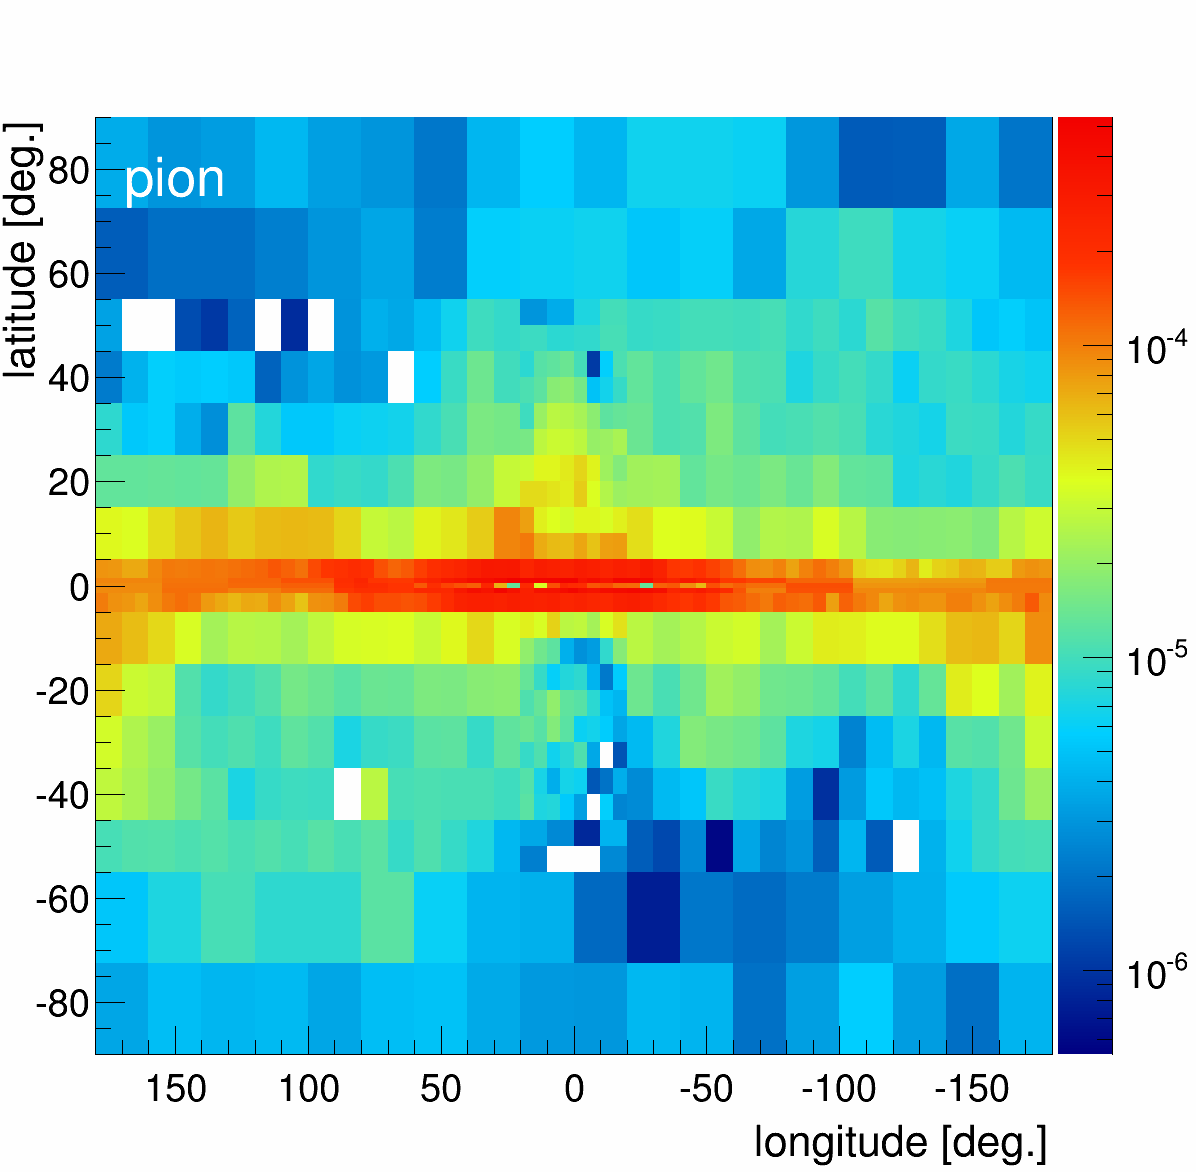
\includegraphics[width=1.\linewidth]{pic/discussion/MCRonly_PCR_integral_flux.png}
  	\subcaption{MCR only fit}
  	\label{}
  \end{minipage}
  \hfill
  \begin{minipage}[h]{0.3\textwidth}
	  \centering
	  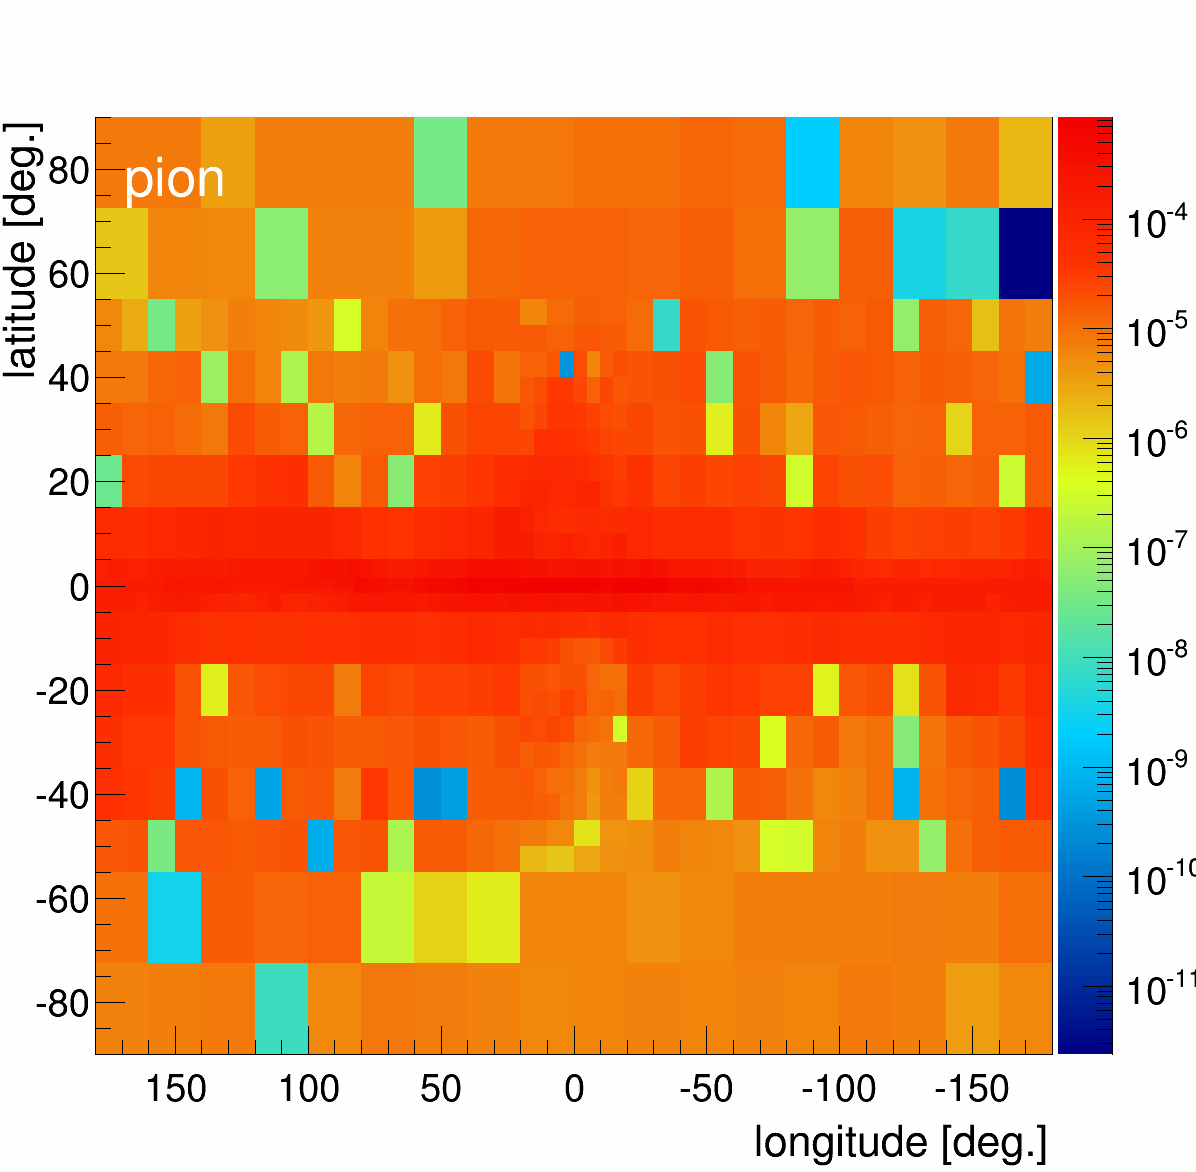
\includegraphics[width=1.\linewidth]{pic/discussion/DMonly_PCR_integral_flux.png}
	  \subcaption{DM only fit}
	  \label{}
  \end{minipage}
  \hfill
  \begin{minipage}[h]{0.3\textwidth}
	  \centering
	  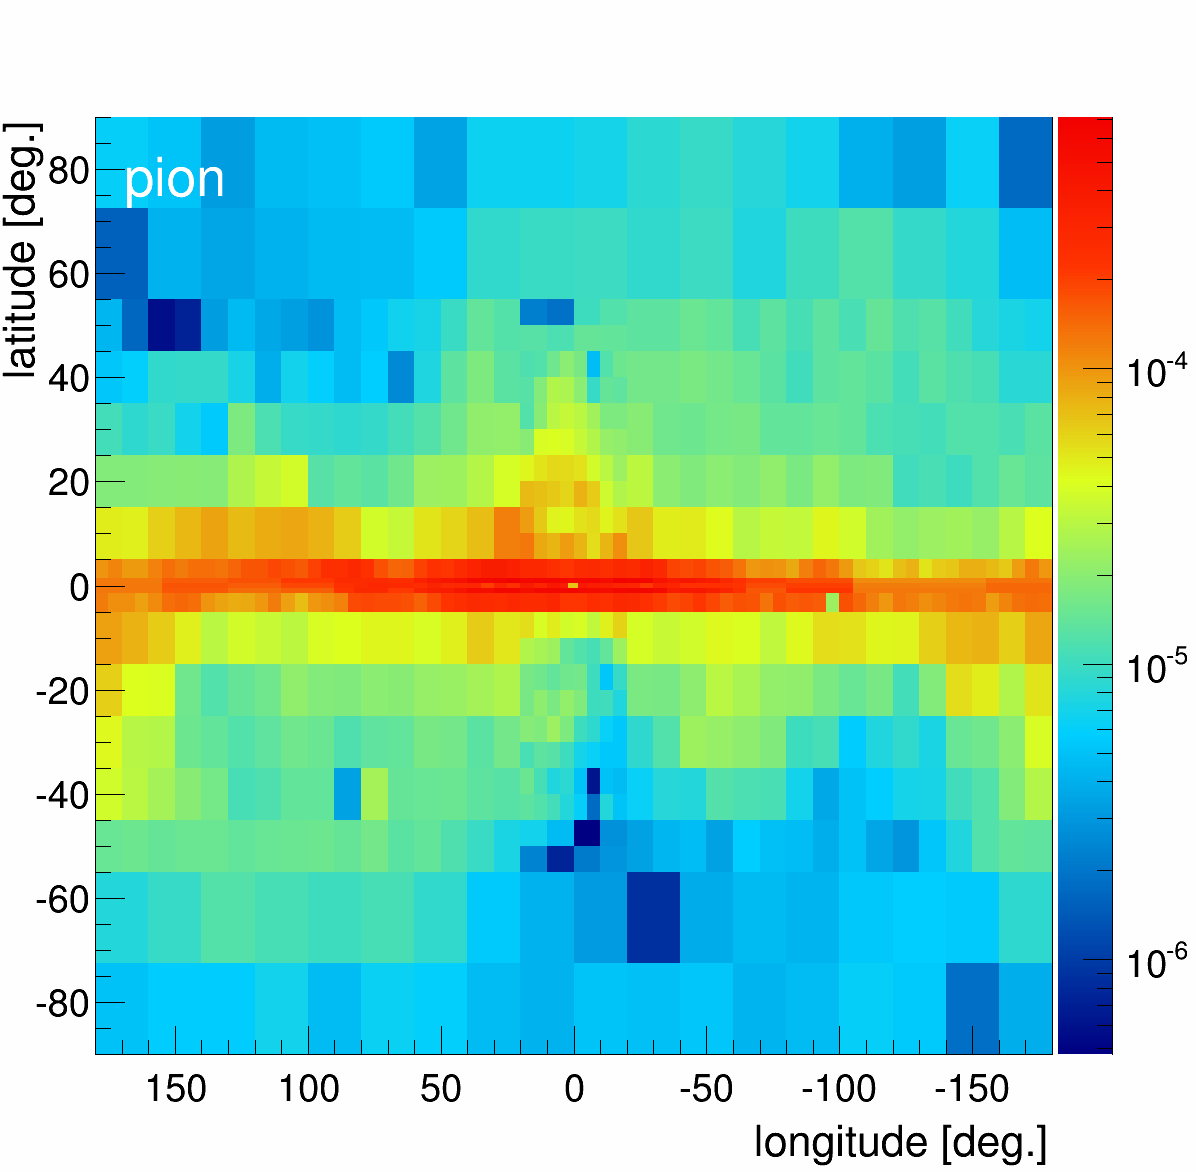
\includegraphics[width=1.\linewidth]{pic/discussion/MSPonly_PCR_integral_flux.png}
	  \subcaption{MSP only fit}
	  \label{}
  \end{minipage}
  \caption{PCR spatial distribution for the three different excess components}
  \label{fig:PCR_flux_distrib_excess_comp}	 
\end{figure}



\subsubsection{IC flux distribution}
The inverse compton component is directly proportional to the ISRF and the electrons CR. Electrons are present everywhere in the galaxy, and the ISRF is dominant in the GC for the UV range, but follows the dust in the IR range and is isotropic in the radio range. This distribution should be visible in the IC component of the fit. Indeed, a spherical distribution can clearly be identified for the three different fits with DM, MCR and MSP.
Nonetheless, there is a noticeable difference int he disk between the IC distribution for the MCR fit and the DM and MSP fits. In the MCR fit, the disk presents a high IC flux when DM and MSP do not. On the contrary, the MSP and DM fit present a clear dip in the galactic disk. This gap is unexpected, since the ISRF is supposed to be the strongest in the disk, and the diffuse electrons are also produced mainly here. \todo{explain this}

\begin{figure}[h]
  \centering
  \begin{minipage}[h]{0.3\textwidth}
  	\centering
	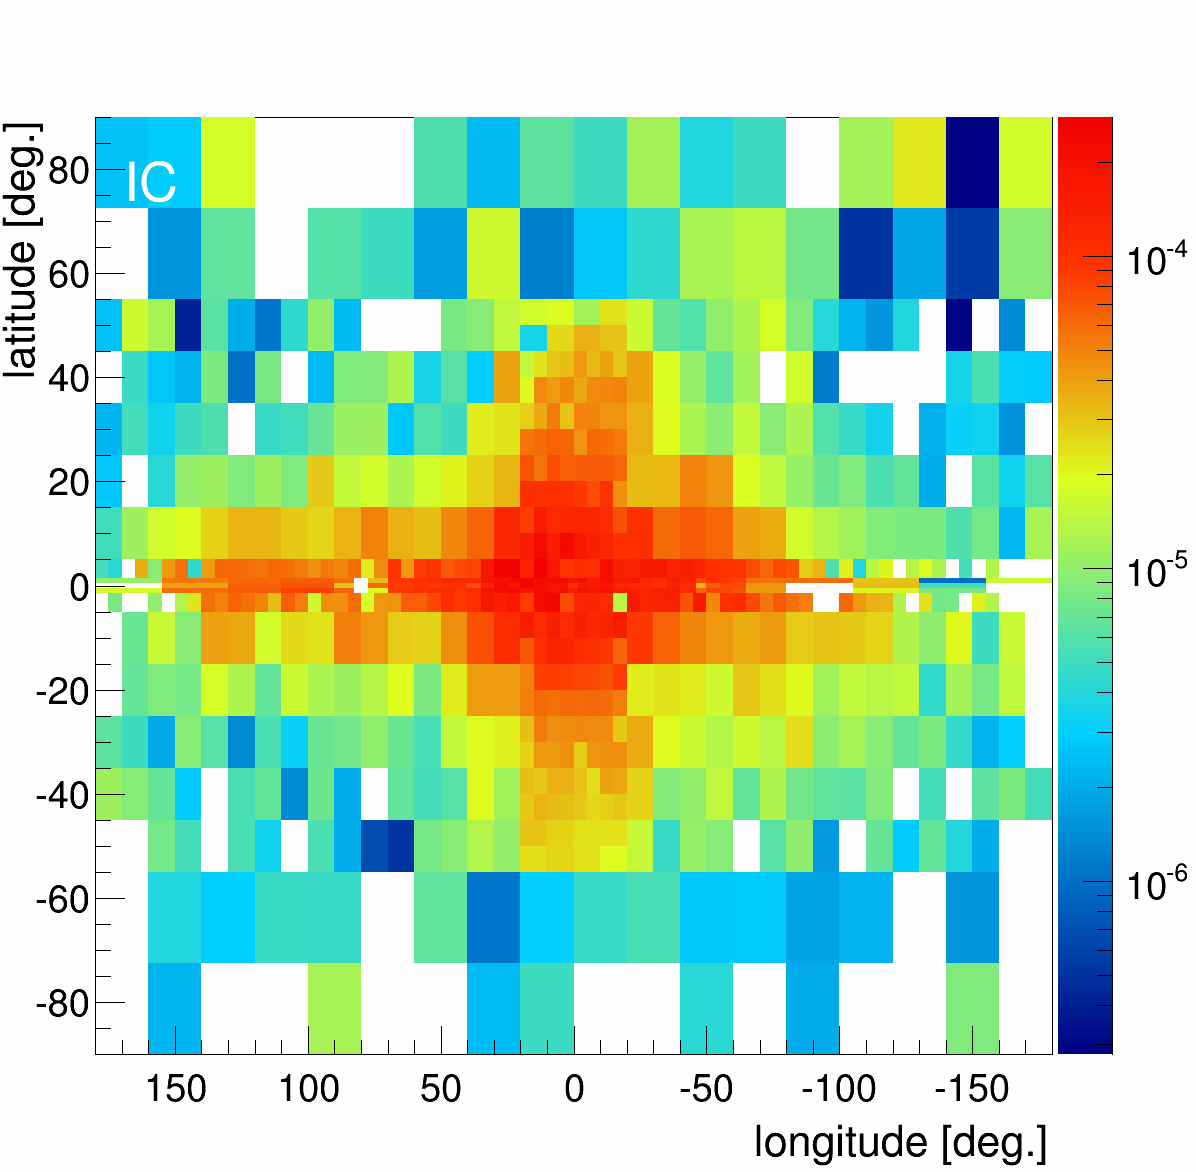
\includegraphics[width=1.\linewidth]{pic/discussion/MCRonly_IC_integral_flux.png}
  	\subcaption{MCR only fit}
  	\label{}
  \end{minipage}
  \hfill
  \begin{minipage}[h]{0.3\textwidth}
	  \centering
	  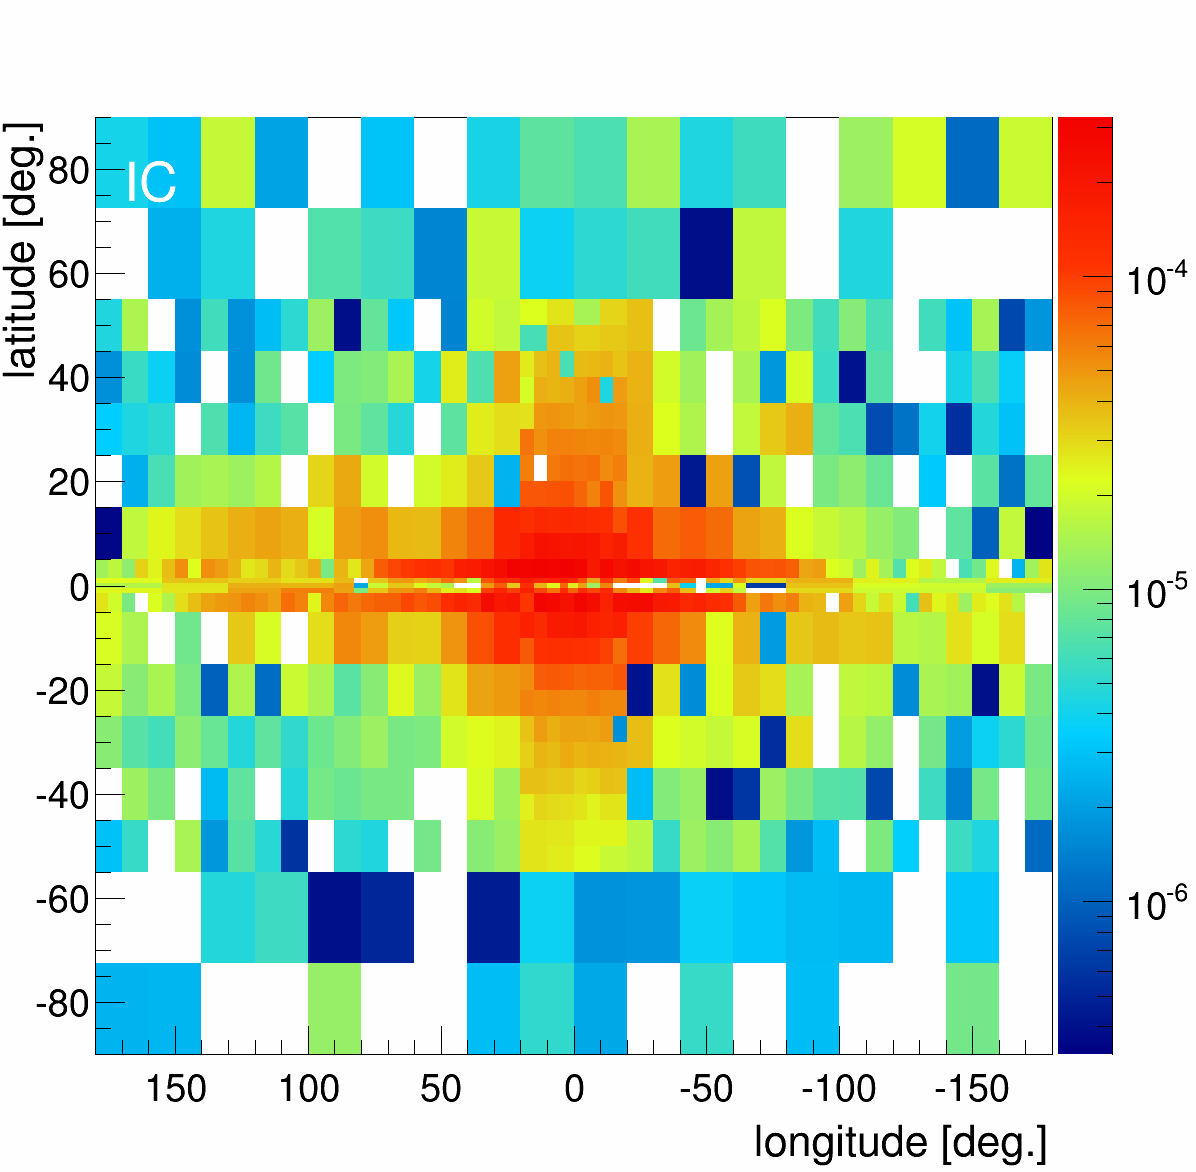
\includegraphics[width=1.\linewidth]{pic/discussion/DMonly_IC_integral_flux.png}
	  \subcaption{DM only fit}
	  \label{}
  \end{minipage}
  \hfill
  \begin{minipage}[h]{0.3\textwidth}
	  \centering
	  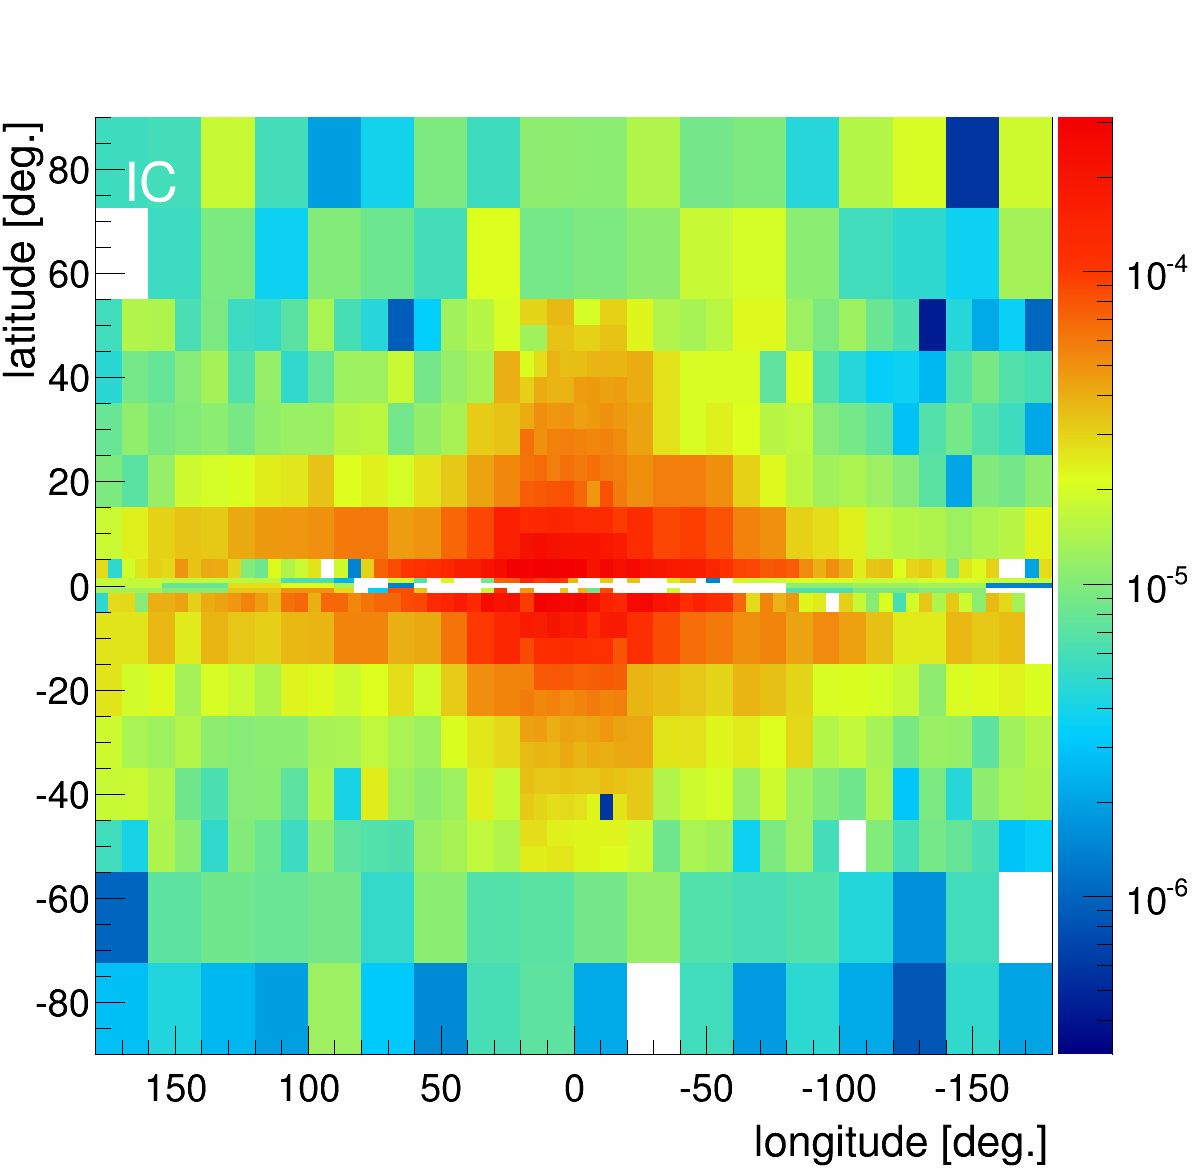
\includegraphics[width=1.\linewidth]{pic/discussion/MSPonly_IC_integral_flux.png}
	  \subcaption{MSP only fit}
	  \label{}
  \end{minipage}
  \caption{IC spatial distribution for the three different excess components}
  \label{fig:IC_flux_distrib_excess_comp}	 
\end{figure}


\subsubsection{BR flux distribution}
The BR component is linked to the CR electron density along the line of sight and the electromagnetic fields in the galaxy. It should then be present everywhere. It is mainly what can be observed here, but some features are remarkable. Mainly the decrease in flux in the disk and the bubbles.
Depending on the fit, the average flux is also changing. The BR component is a lot more present with the MCR fit than with DM, which in turn presents more BR than the MSP fit. The fact that the MSP fit does not use a lot of BR is consistent with the fact that the MSP spectrum is very soft at low energies. Since BR is also dominant at these energies, both can not have a high flux at the same time. The fit must do concession in order to use them both.

\begin{figure}[h]
  \centering
  \begin{minipage}[h]{0.3\textwidth}
  	\centering
	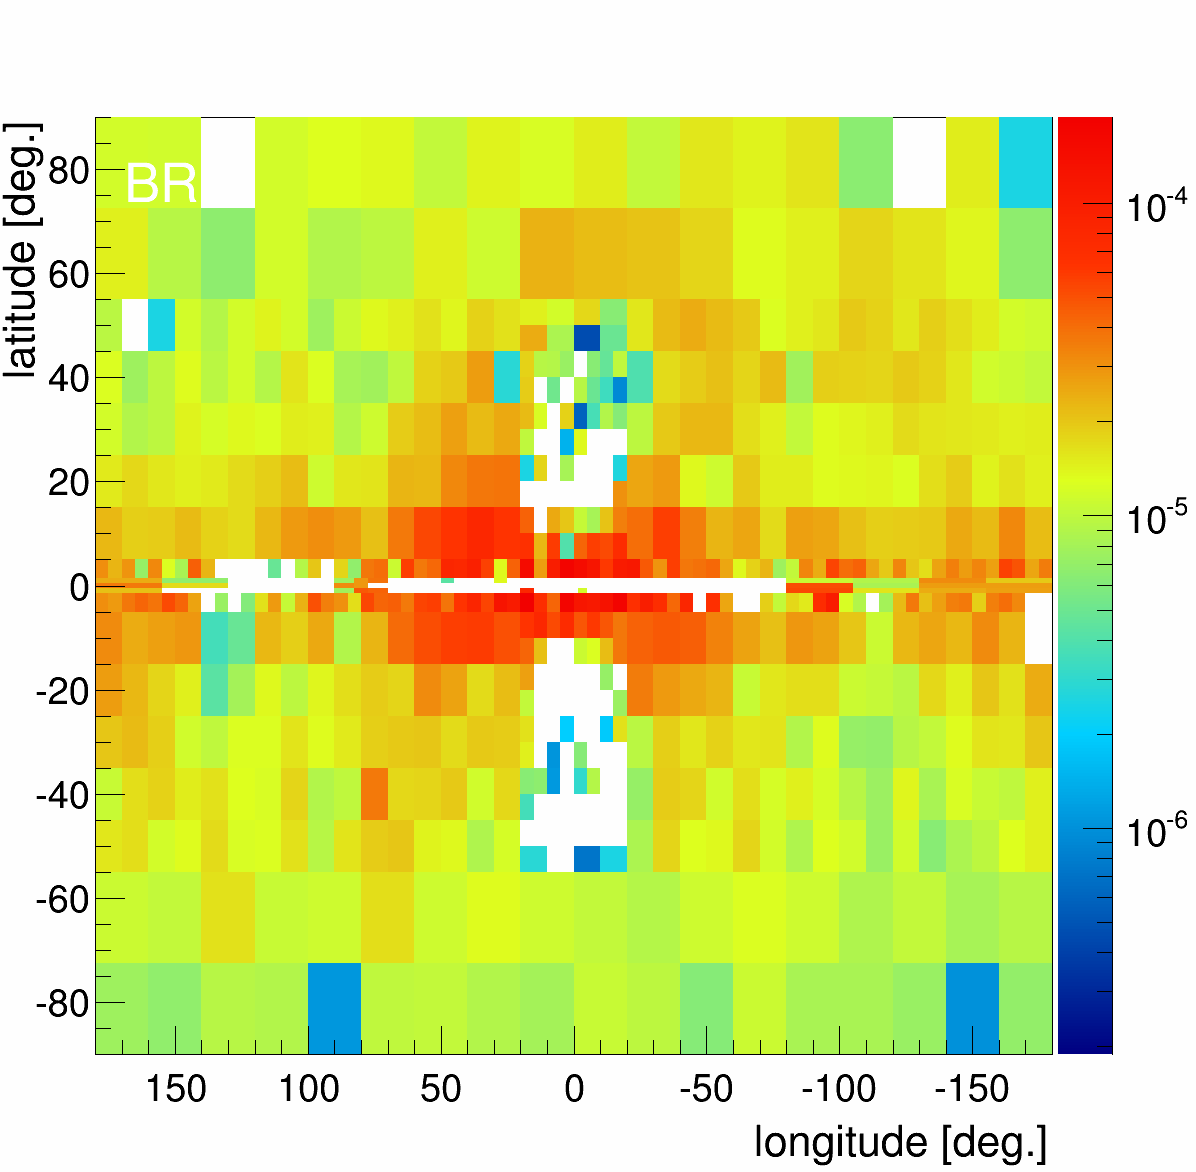
\includegraphics[width=1.\linewidth]{pic/discussion/MCRonly_BR_integral_flux.png}
  	\subcaption{MCR only fit}
  	\label{}
  \end{minipage}
  \hfill
  \begin{minipage}[h]{0.3\textwidth}
	  \centering
	  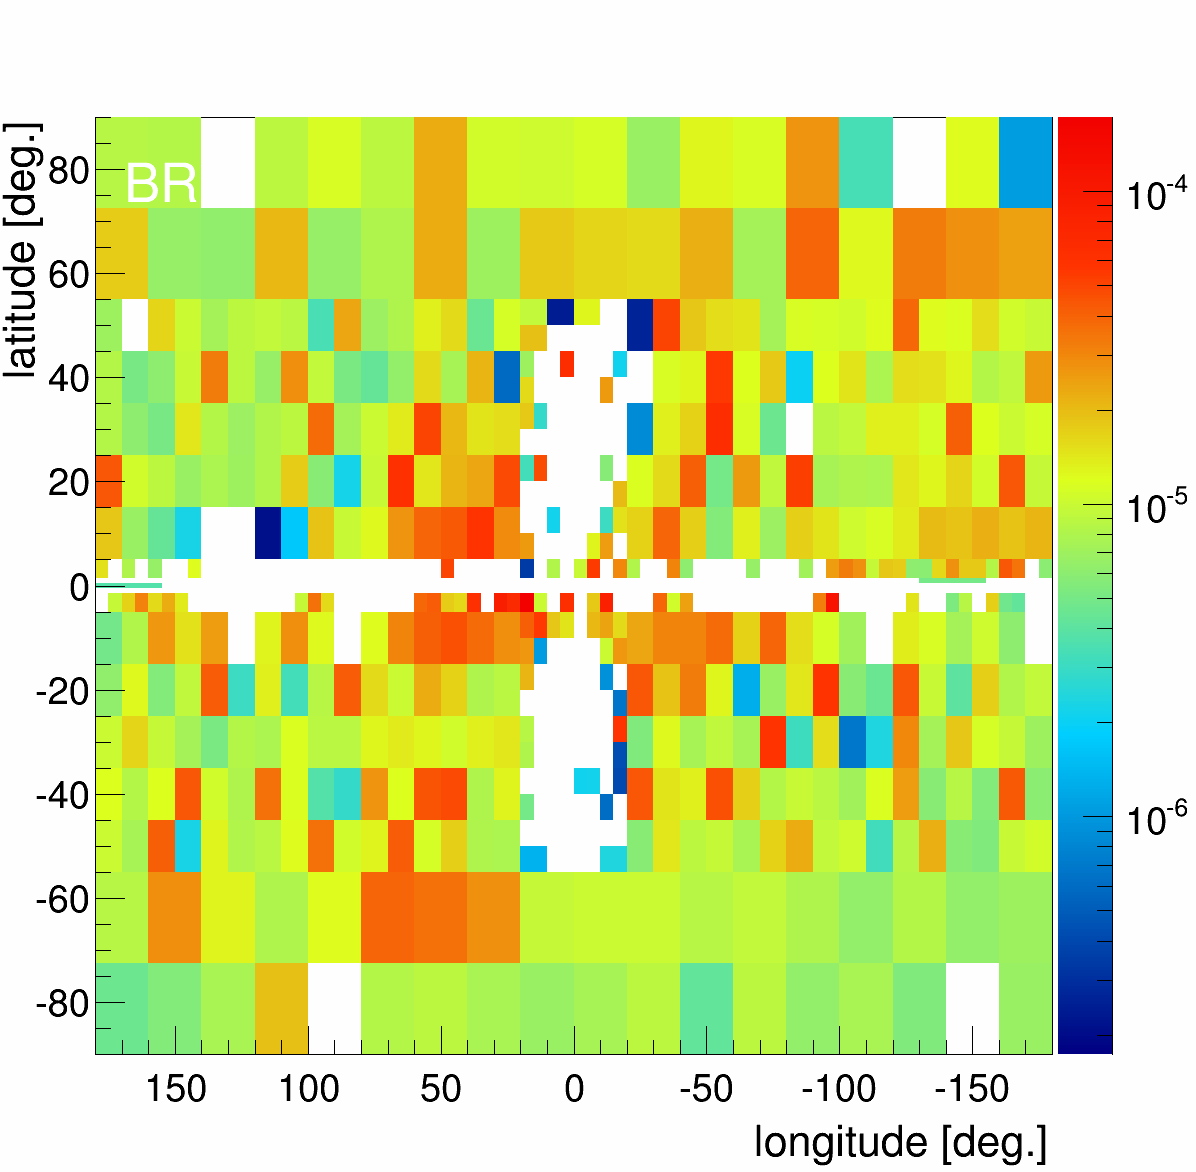
\includegraphics[width=1.\linewidth]{pic/discussion/DMonly_BR_integral_flux.png}
	  \subcaption{DM only fit}
	  \label{}
  \end{minipage}
  \hfill
  \begin{minipage}[h]{0.3\textwidth}
	  \centering
	  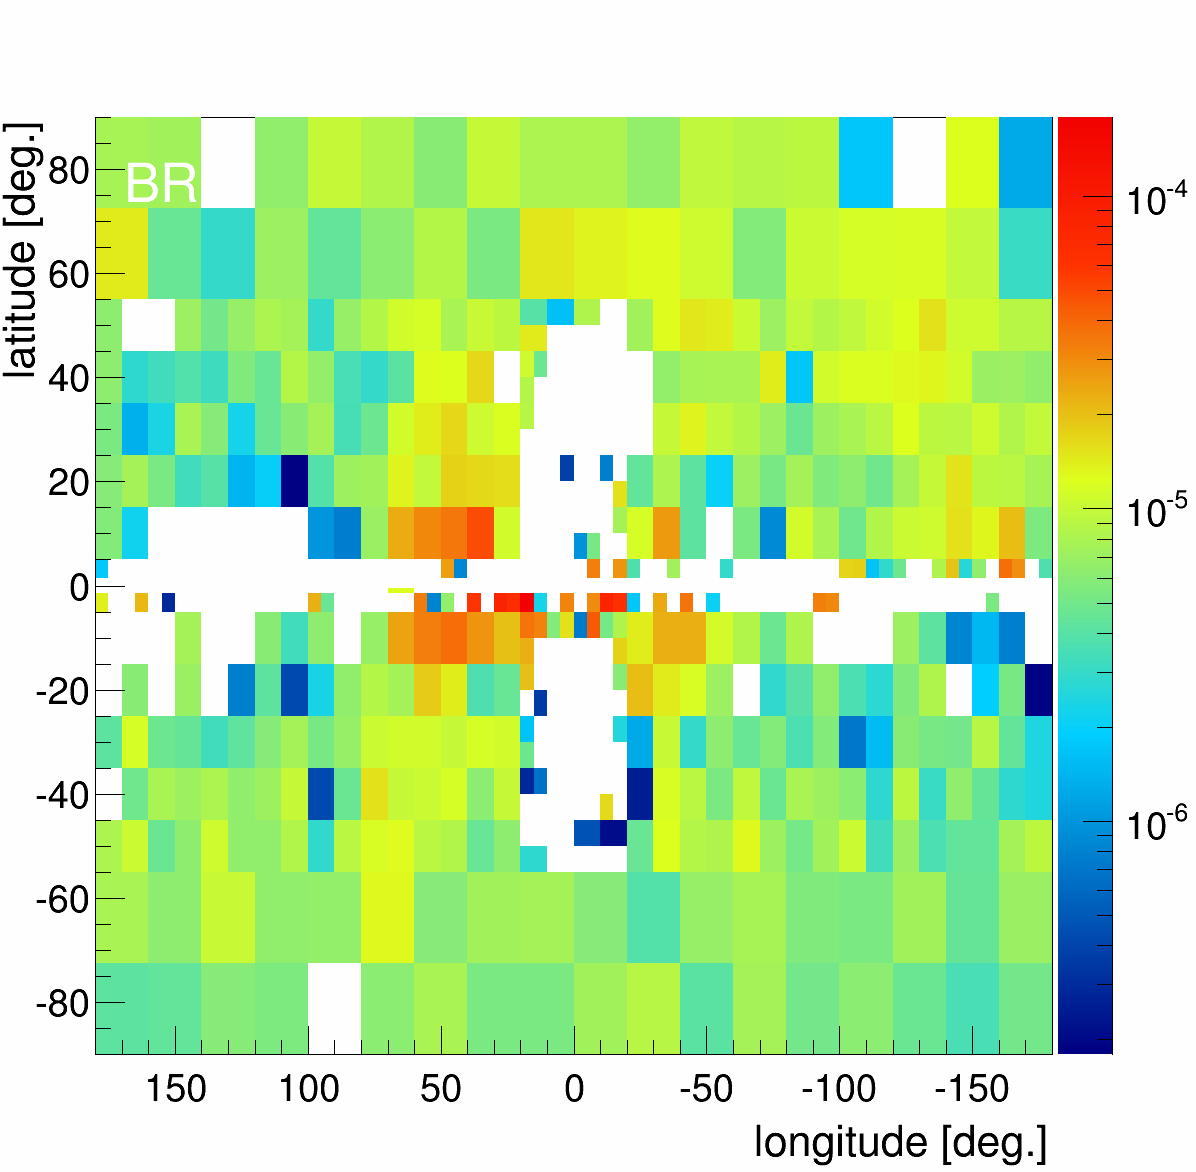
\includegraphics[width=1.\linewidth]{pic/discussion/MSPonly_BR_integral_flux.png}
	  \subcaption{MSP only fit}
	  \label{}
  \end{minipage}
  \caption{BR spatial distribution for the three different excess components}
  \label{fig:BR_flux_distrib_excess_comp}	 
\end{figure}

\subsubsection{SCR flux distribution}
The SCR distribution is expected to follow the disc, where point sources can still remains, and the bubbles, where the proton CR spectra is harder. And indeed, the spatial distribution obtained in the three  different fits are similar and correspond perfectly to the expectations.


\begin{figure}[h]
  \centering
  \begin{minipage}[h]{0.3\textwidth}
  	\centering
	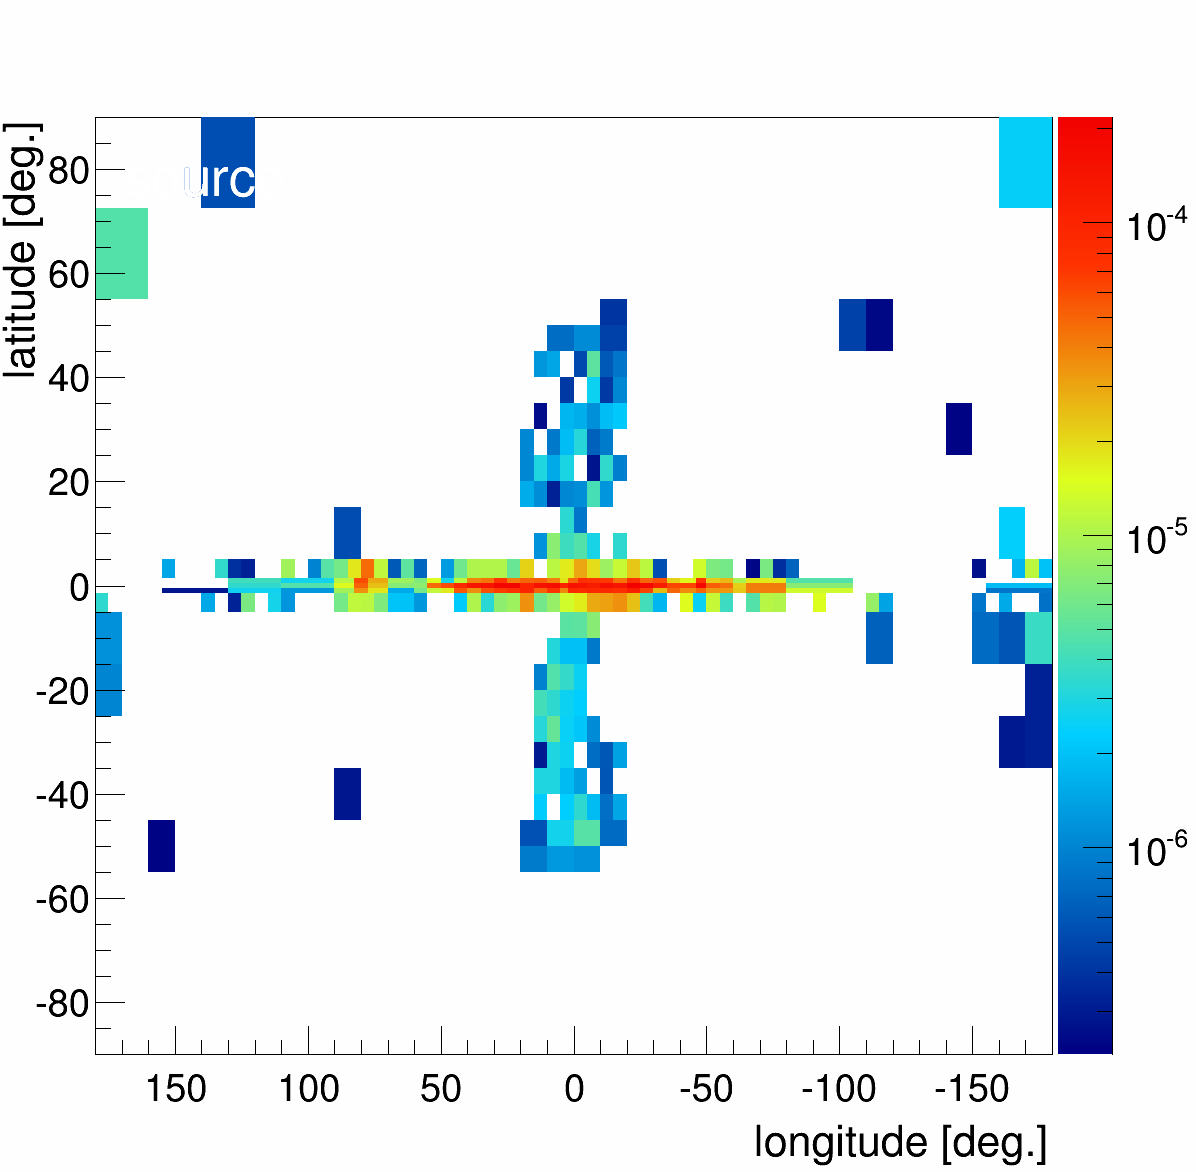
\includegraphics[width=1.\linewidth]{pic/discussion/MCRonly_SCR_integral_flux.png}
  	\subcaption{MCR only fit}
  	\label{}
  \end{minipage}
  \hfill
  \begin{minipage}[h]{0.3\textwidth}
	  \centering
	  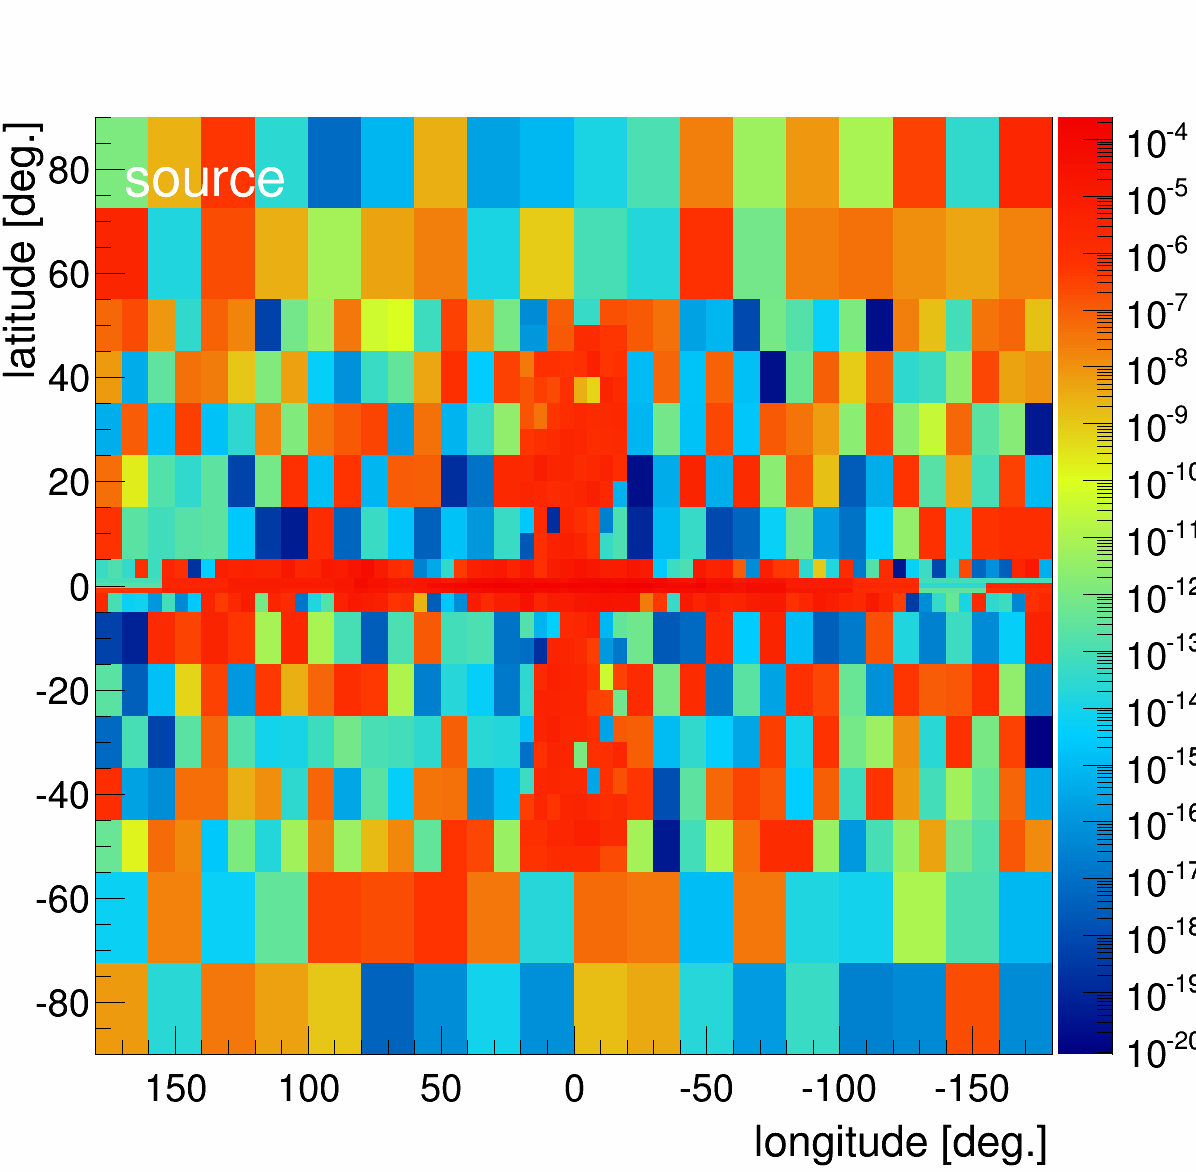
\includegraphics[width=1.\linewidth]{pic/discussion/DMonly_SCR_integral_flux.png}
	  \subcaption{DM only fit}
	  \label{}
  \end{minipage}
  \hfill
  \begin{minipage}[h]{0.3\textwidth}
	  \centering
	  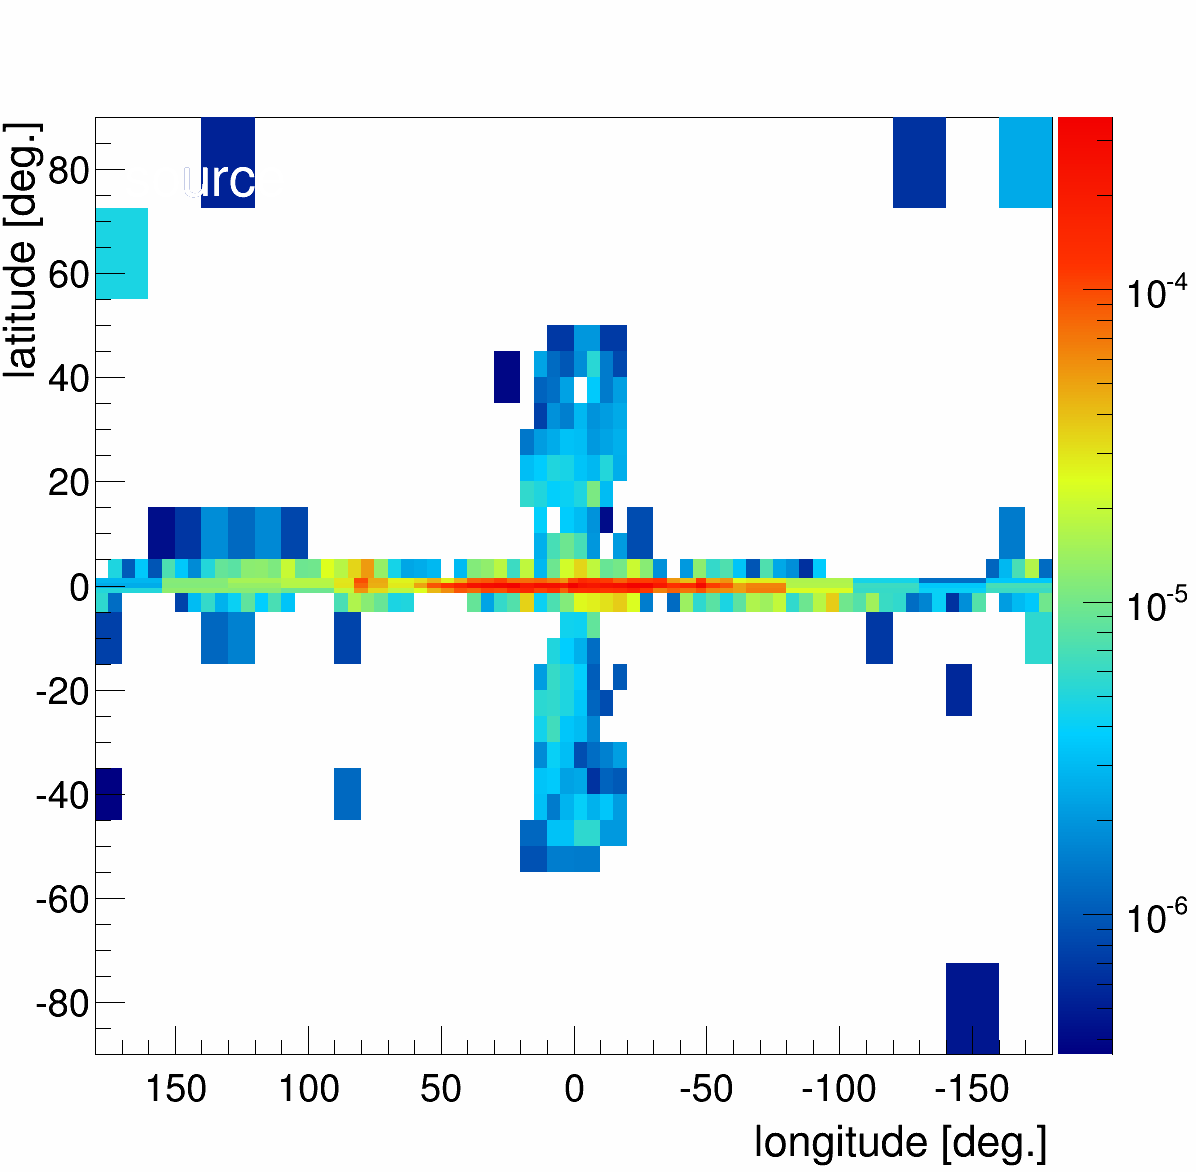
\includegraphics[width=1.\linewidth]{pic/discussion/MSPonly_SCR_integral_flux.png}
	  \subcaption{MSP only fit}
	  \label{}
  \end{minipage}
  \caption{SCR spatial distribution for the three different excess components}
  \label{fig:SCR_flux_distrib_excess_comp}	 
\end{figure}


\section{Adding the MBR component}

\subsection{MBR fixed to MCR, magnetic cut-off}
\todo{add pictutures of graph and skymaps}

The theory behind the MCR component involves a magnetic cut-off for low rigidity CR protons, that changes the gamma-ray spectrum at low energies. Such a cut-off only depends on the rigidity of the CR and the intensity of the electromagnetic field. So there is no reason for it to be only applied to protons, and not to electrons. This is the reasoning that led to introducing a new template, called MBR in the fit, equivalent to the BR template, but calculated from a different electron CR spectra. This new CR spectra present two parts, with two different power laws for high or low energies. It has the exact same spectral indexes than the spectrum for IC and BR, but the break is moved up between 6 and 14 GeV. Then, the break is taken to have the same value than the MCR brake. This way, the magnetic cut-off is applied the same way to the electrons and protons CR. Once again, this component is expected to follow the MCs distribution, or at least to be only present in the disk.

A MIC component was tested as well, but it was not kept for physical reasons. First, the ISRF is not dependent of the electromagnetic field, photons do not carry any electric charge. It is also present in MC, where stars are formed and evolve.

%\subsection{MBR free, Alfen waves}



\section{Add DM late}

\todo{difference with DM+MCR. Results and discussion.}

Now the results are clear. MCR is a good solution to the gamma-ray GeV excess in the GC, and could replace the first hypothesis of the DM halo or hidden MSPs. Yet, the DM theory is strongly supported by other measurements \todo{cite}, for example the rotation curves of galaxies, and is one of the most important question of modern physics. And the fact that it is not the primary cause of the effect observed here does not mean it does not exist. On the contrary, under the hypothesis that MCR is really the cause of the excess, the fit could put strong limits on the DM models.

This section will present a few ways to study the current DM WIMP model using the fit method of this thesis.

\subsection{DM and MCR}

\todo{add figure}
A first idea is to let the fit choose for every cone the template that offers the best $\chi^2$ value. Taking a 52.3 GeV WIMP mass and the MCR template with free breaks, the fit has the choice between the two. The results are without much surprise in favor of MCR. Indeed, the previous comparisons of the $\chi^2$ distribution for a MCR or a DM fit showed a clear preference toward MCR. The $\chi^2$ map of a MCR fit is flat around one, even in the disk, whereas a DM fit does not work well for small latitudes. It is then only expected that the fit chooses MCR when it has the choice.

\subsection{DMlate}

This method can not say much else than what was already showed in the previous sections. The second idea that comes to mind is to take the MCR template for granted, and see if their is space to add DM contribution at the end of the fit. In other words, a first fit is performed with the classical templates (PCR, IC, BR), the source (SCR) and the MCR templates. Once the best relative contributions are found, the fit tries to add a DM template to improve the $\chi^2$.
Following the Ockham's razor principle, the least amount of contributions are accepted as true, and any additional component must be treated carefully. This way, the necessity of a DM template is checked, and it contribution can not be mistaken for a classical one.
\todo{add pic}
Such a fit was performed and the results will be discussed in this section. First of all, the DM flux distribution  is very sparse and degrees of magnitude below the other components. This was expected since the $\chi^2$ of the MCR only fit was already good. Only very small changes could improve it without changing the classical contributions. Using the same CMZ region in the GC, the optimal mass was determined to be \todo{mass DM late}.

Further studies of this kind could help to determine limits on the DM particle mass and cross-section.


\section{How do these results fit in context}
%How do they fit in context:
%	-DM explanation
%		-Best mass around 50 GeV
%		-Increase goodness of fit
%		-Not spherical at all
%		-Follows CO map when there is no reason to do it
%	-MSP explanation
%		-Spectra too soft at low energies.
%		-Same problem than with DM.
%		
%	-What's new?






